\documentclass[tikz,border=5pt]{standalone}
\usepackage{pgfplots}
\pgfplotsset{compat=1.18}
\usepackage{fontspec}
\setsansfont{SourceSansPro}[
  Path = /usr/local/texlive/2024/texmf-dist/fonts/opentype/adobe/sourcesanspro/,
  UprightFont = SourceSansPro-Regular.otf,
  BoldFont = SourceSansPro-Bold.otf,
  ItalicFont = SourceSansPro-RegularIt.otf,
  BoldItalicFont = SourceSansPro-BoldIt.otf,
  Scale = 1.0
]
\usetikzlibrary{positioning}
\usepackage{xcolor}
\definecolor{primaryblue}{HTML}{012169}
\definecolor{primarygold}{HTML}{B9975B}
\definecolor{highlightyellow}{HTML}{F2A900}
\definecolor{lightbg}{HTML}{E8EDF5}
\definecolor{jet}{HTML}{1A1A1A}
\definecolor{positivegreen}{HTML}{15803D}
\definecolor{negativered}{HTML}{B91C1C}
\begin{document}
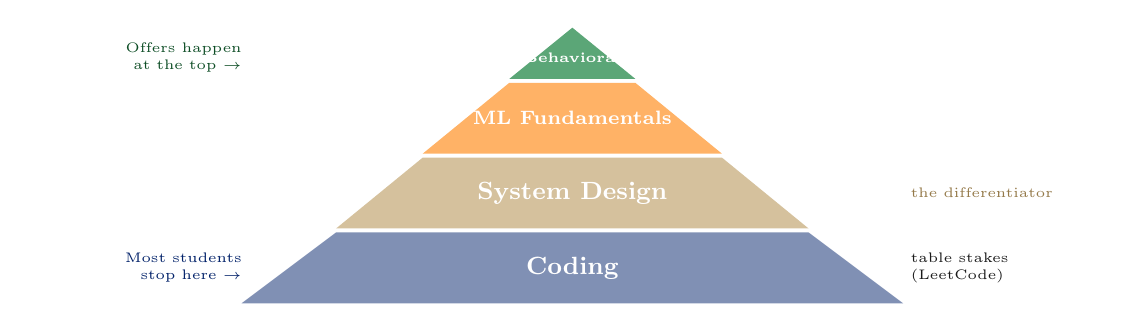
\begin{tikzpicture}[scale=1.0]
  % Layer 1 — bottom: Coding (widest)
  \fill[primaryblue!50]  (-4.2,0)    -- (4.2,0)    -- (3.0,0.9)  -- (-3.0,0.9)  -- cycle;
  % Layer 2: System Design
  \fill[primarygold!60]  (-3.0,0.95) -- (3.0,0.95) -- (1.9,1.85) -- (-1.9,1.85) -- cycle;
  % Layer 3: ML Fundamentals
  \fill[orange!60]       (-1.9,1.9)  -- (1.9,1.9)  -- (0.8,2.8)  -- (-0.8,2.8)  -- cycle;
  % Layer 4 — top: Behavioral
  \fill[positivegreen!70](-0.8,2.85) -- (0.8,2.85) -- (0,3.5)    -- cycle;
  % Inside labels (short)
  \node[font=\small\bfseries, text=white]          at (0,    0.45) {Coding};
  \node[font=\small\bfseries, text=white]          at (0,    1.40) {System Design};
  \node[font=\scriptsize\bfseries, text=white]     at (0,    2.35) {ML Fundamentals};
  \node[font=\tiny\bfseries,       text=white]     at (0,    3.12) {Behavioral};
  % Right-side descriptions
  \node[font=\tiny, text=jet, align=left, text width=2.4cm]
        at (5.5, 0.45)  {table stakes\\(LeetCode)};
  \node[font=\tiny, text=primarygold!80!black, align=left, text width=2.4cm]
        at (5.5, 1.40)  {the differentiator};
  % Left-side callouts
  \node[font=\tiny, text=primaryblue, align=right, text width=2.6cm]
        at (-5.5, 0.45)  {Most students\\stop here $\rightarrow$};
  \node[font=\tiny, text=positivegreen!60!black, align=right, text width=2.6cm]
        at (-5.5, 3.12) {Offers happen\\at the top $\rightarrow$};
\end{tikzpicture}
\end{document}
